\chapter{Characterization: How we measured the actual grating performance, and accounted for differences}
In the previous chapter, we applied grating efficiency calculations to create and optimize the optical design of the REIXS emission spectrometer.  After having the design reviewed by an external consultant, who confirmed our resolution and efficiency predictions (TODO REF), we solicited bids from grating manufacturers and selected Bach Research to mechanically rule the six gratings.  Finally, we passed the optical requirements over to a consulting engineer to design the mechanics of the spectrometer, which would be responsible for positioning the entrance slit, gratings, and detector, as well as achieving and maintaining ultra-high vacuum conditions throughout the beam path.

We lamented back in Chapter 4 the lack of published experimental comparisons of grating efficiency -- particularly in the soft x-ray regime -- and hypothesized that this was because beamline scientists, on receiving new gratings, were often eager to put them into their beamline and start commissioning, rather than spend more time characterizing them.  Unfortunately\footnote{for us in our role as beamline staff}, the construction of the REIXS spectrometer was delayed by a series of serious mechanical design flaws and oversights.  Fortunately\footnote{for our interests in grating efficiency}, this setback provided us with lots of time to characterize the ruling quality and real-world diffraction efficiency of our gratings.  Even more fortunately, the characterization process alerted us to serious ruling errors with a few of the gratings, which would have dramatically affected the spectrometer's resolution and efficiency had they not been discovered.  In the end, our characterization of the gratings resulted in several beneficial outcomes:
\begin{itemize}
\item We were able to contribute another set of experimental comparisons to theoretical grating efficiency calculations.
\item We discovered a reason to be cautious when specifying nickel-coated gratings, despite nickel's apparently high reflectivity.
\item We discovered a serious ruling problem in the HEG grating, which nearly eliminated its ability to diffract in the useful orders, and sent it back to the manufacturer for re-coating and re-ruling.
\item We discovered substantial errors in the blaze angle (beyond the manufacturer's specified tolerance) for a few of the gratings; in the case of the HRHEG, the blaze angle was off by so much that we ended up using it as a temporary replacement for the HEG.
\end{itemize}

This chapter describes these results, based on atomic force microprobe (AFM) measurements of the groove profile and soft x-ray diffractometer measurements of the actual grating efficiency.  We also compare the calculated and measured grating efficiencies, and offer explanations for the differences.

\section{AFM measurements of the manufactured grating profile}
When we consider a grating like the HEG, with 2000 lines/mm and a blaze angle of 1.52$\deg$, it is clear that the physical size of the grooves is extremely small -- these are little triangles about 500 nm wide and maybe 13 nm tall.  Measuring the physical geometry is therefore actually impossible with a visible light microscope.

Instead, we used atomic force microscopy (AFM), an extremely high-resolution technique for measuring the topography of a surface.  It uses an extremely sharp-tipped mechanical probe mounted on a piezo-electrically-controlled cantilever to ``feel'' the surface (Figure \ref{afm}).  The tip can either be dragged across the surface (contact mode) or electronically oscillated near its resonance frequency (\emph{non-contact mode}) while measuring the change in amplitude, phase and frequency caused by the tip-sample atomic interaction forces.  In both cases, the accurate vertical position of the tip is measured with a laser beam reflected off the back of the cantilever -- using either an interferometer or a deflection meter -- and the horizontal position of the tip is scanned using piezo drivers.  The resolution of the best atomic force microscopes is sufficient to image individual atoms on a surface, although for measuring soft x-ray gratings we only need angstrom-level accuracy.

One limitation of AFM techniques is that it is easy to produce a two-dimensional map of the relative surface profile in arbitrary units, but difficult to accurately determine the absolute height.  In order to measure blaze angles of gratings, we need to measure the height difference from the bottom to the top of the grooves in absolute units, which requires calibration of the AFM using a height standard.  (Usually this is a gold mesh with an accurately-known wire size.)

After receiving the gratings from the manufacturer, we first imaged them using the AFM at the University of Saskatchewan Structural Sciences Centre (SSSC).  However, we were not able to calibrate the $z$-axis for these measurements, so with the assistance of Dr. Eric Gullikson, we requested a complete set of measurements using the AFM at the Center for X-Ray Optics at the Lawrence Berkeley National Laboratory.

An example of an AFM scan is given in Figure \ref{5a}, where we show both the two-dimensional image (top) and a cross-section of heights perpendicular to the grooves (bottom), which reveals the groove profile.  Although the grooves should be ideally uniform along their entire length, most of the AFM scans show profile variation across even one image (a distance of just a few micrometers).  To determine the average profile shape and average blaze angle, we integrated the two-dimensional image across the groove direction.  Since a single AFM scan only spans a few micrometers of the grating, we also need to be careful in extrapolating the results to the entire grating; therefore, we conducted multiple scans at the centre and the corners of the grating.

Figure \ref{5a} gives an example of the AFM output, for the LEG grating.  We present  groove profiles for all the gratings starting in Section \ref{gratingResults}, alongside a discussion of their effective diffraction performance.

\begin{figure}[htbp] %  figure placement: here, top, bottom, or page
   \centering
   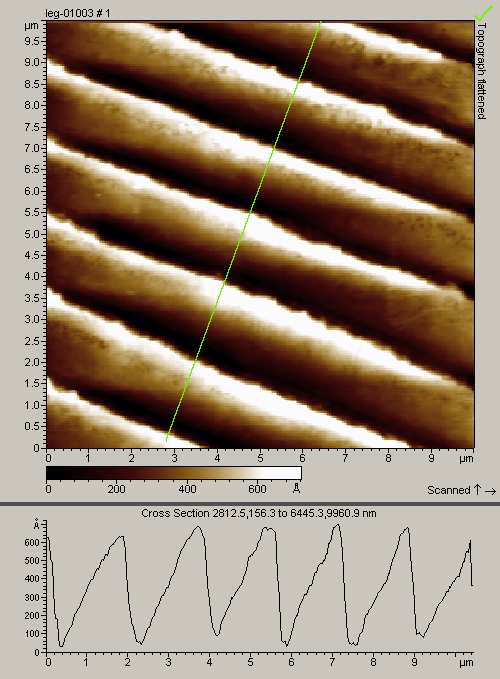
\includegraphics[scale=0.25]{Chapter5/5a_exampleAFM/afm_LEG_xsect1.png} 
   \caption{The Low Energy Grating has a smooth regular profile, shown in this example image measured using an Atomic Force Microprobe (AFM).}
   \label{5a}
\end{figure}

\section{Diffractometer measurements of actual grating efficiency}
To measure the actual grating efficiency, we used the reflectometer on the Calibration and Standards Beamline (6.3.2) at the Advanced Light Source.  This beamline was designed specifically for testing the reflectivity of soft x-ray optical components like mirrors, thin films, multilayer coatings, and gratings.  It consists of a bending magnet source, a VLS-PGM monochromator with a resolving power of 7000 (Figure \ref{5b-a}), a higher-order suppressor, and a two-circle reflectometer (Figure \ref{5b}).  The beamline optics can focus the monochromator light to a small spot on the sample, or focus at infinite to generate parallel light (TODO REF http://ieeexplore.ieee.org/xpl/freeabs\_all.jsp?arnumber=4994440).

\begin{figure}[htbp] %  figure placement: here, top, bottom, or page
   \centering
   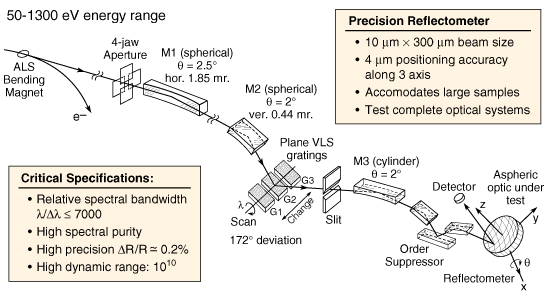
\includegraphics[scale=0.8]{Chapter5/5b_diffractometer/beamlineSchematic2.png} 
   \caption[The Calibration and Standards Beamline (6.3.2) at the Advanced Light Source consists of a bending magnet source, a VLS-PGM monochromator with three selectable gratings, a higher-order suppressor, and a two-circle reflectometer.]{The Calibration and Standards Beamline (6.3.2) at the Advanced Light Source consists of a bending magnet source, a VLS-PGM monochromator with three selectable gratings, a higher-order suppressor, and a two-circle reflectometer shown in more detail in Figure \ref{5b}.  The curvature of refocussing mirror M3 can be adjusted to image the exit slit onto the sample, or to focus the light at infinite.  \textbf{Image from}: (TODO REF http://cxro.lbl.gov/als632/)}
   \label{5b-a}
\end{figure}

\subsection{Beamline 6.3.2 reflectometer}

\begin{figure}[htbp] %  figure placement: here, top, bottom, or page
   \centering
   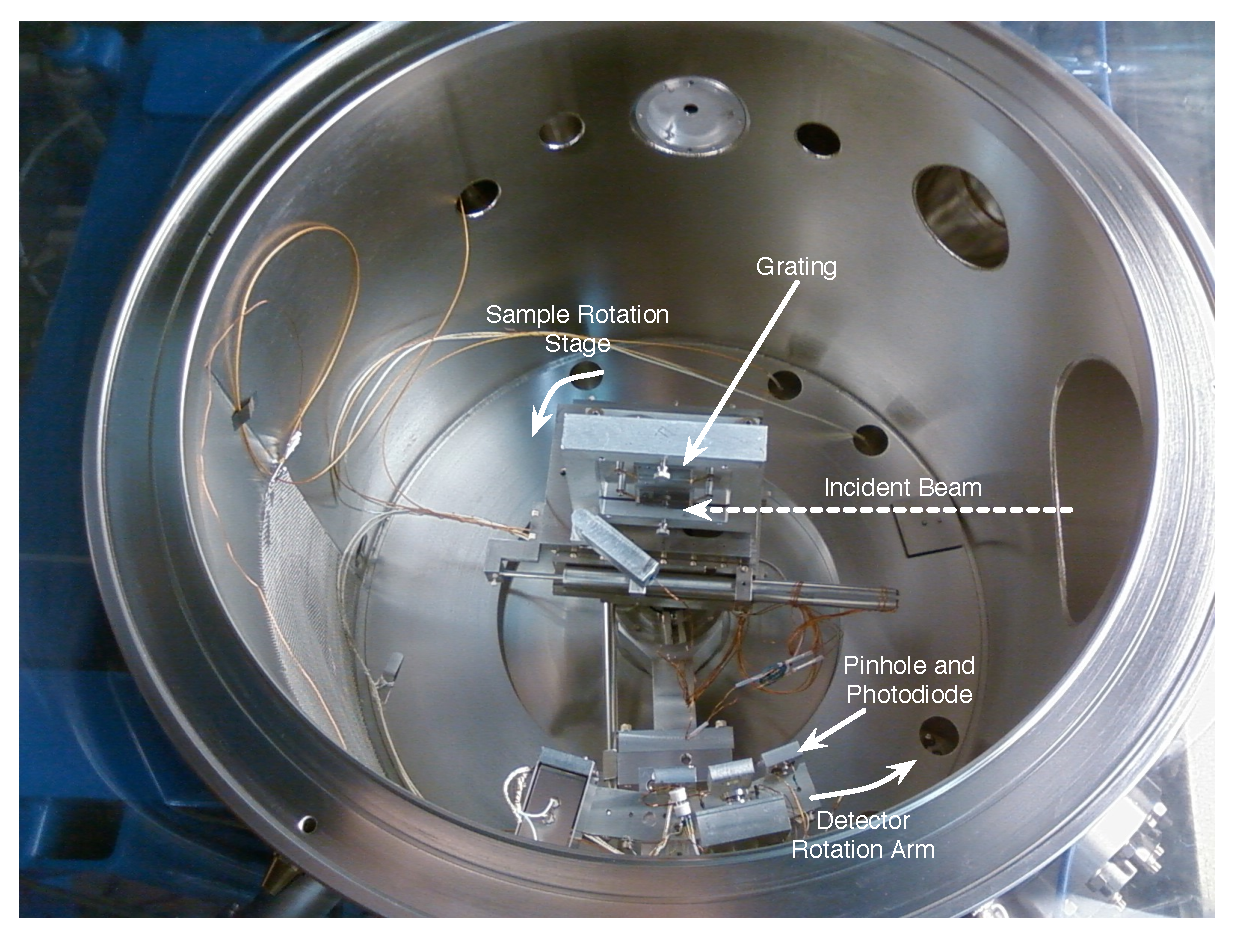
\includegraphics[scale=0.8]{Chapter5/5b_diffractometer/diffractometerLabelled2.pdf} 
   \caption[The reflectometer on Beamline 6.3.2 at the Advanced Light Source allows for independently setting the angle of the gratings in the beam, and setting the angle of a pinhole photodiode detector.]{The reflectometer on Beamline 6.3.2 at the Advanced Light Source allows for independently setting the angle of the gratings in the beam, and setting the angle of a pinhole photodiode detector.  Upstream, filters in the beamline are used to remove contamination from the higher-order light of the monochromator. }
   \label{5b}
\end{figure}

The purpose of the reflectometer endstation (Figure \ref{5b}) is to measure the intensity of light reflected off a sample -- in our case, a grating -- as a function of both incidence and reflection angle.  We used it to determine grating efficiency by positioning the grating at the intended incidence angle relative to the incoming beam,  measuring the intensity at the angle of the outgoing order, and comparing this to the initial beam intensity.  Upstream, the monochromator and order suppressor were used to produce the monochromatic incident beam and set its energy for each datapoint.

\begin{figure}[htbp] %  figure placement: here, top, bottom, or page
   \centering
   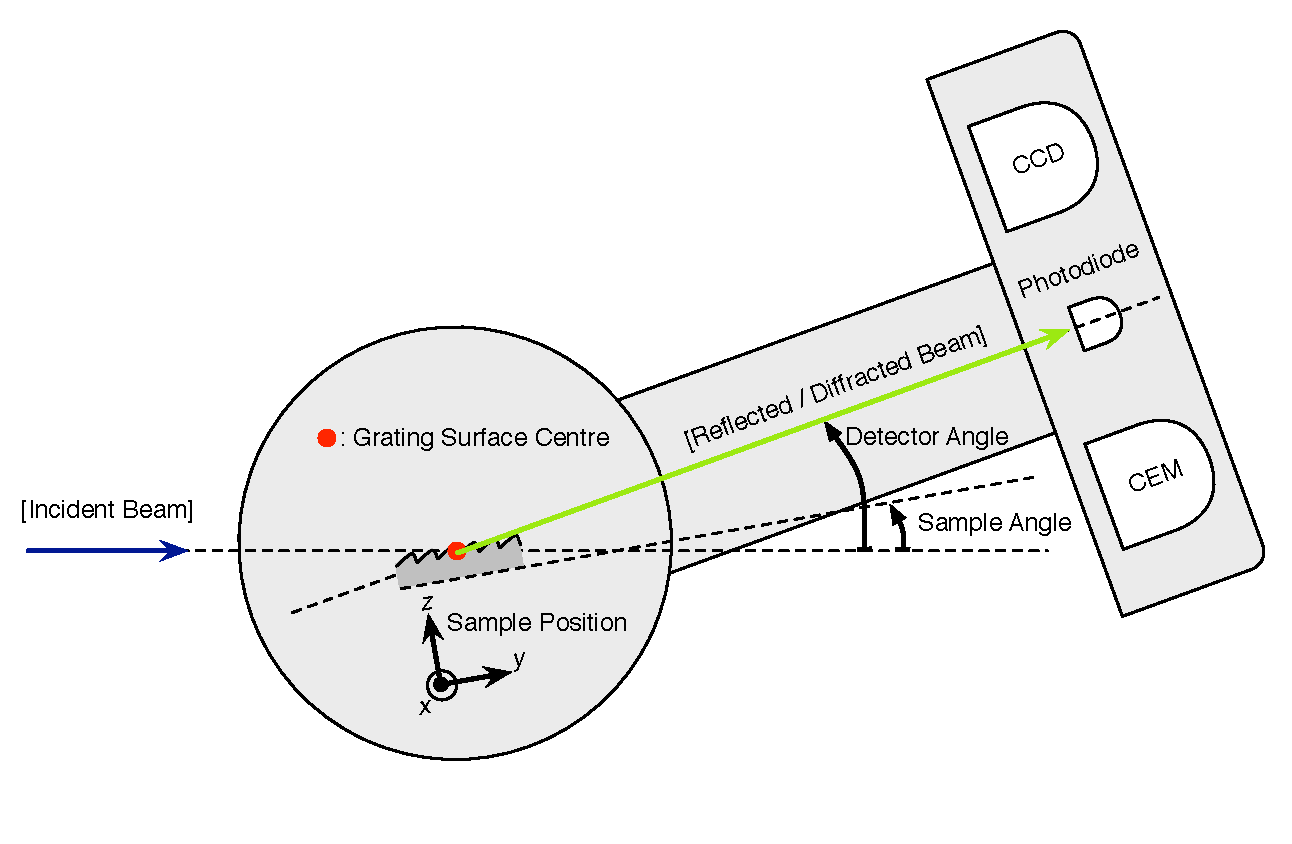
\includegraphics[scale=0.8]{Chapter5/5b_diffractometer/reflectometerCoordinates.pdf} 
   \caption[Reflectometer coordinates: the sample angle is measured up from grazing incidence, and the detector angle is measured up from grazing incidence.]{In the coordinate convention for the reflectometer, the sample angle is measured up from grazing incidence, and the detector angle is measured up from grazing incidence.  The sample position stage ($x$, $y$, $z$) is mounted to the sample angle stage, so that the centre of rotation is always at the height of the beam.}
   \label{reflectometerCoordinates}
\end{figure}

Inside the reflectometer mechanics, a ``two-circle goniometer'' provided independent control over the angle of the sample and the angle of the detector arm, as well as providing precise (4 um) positioning to align the sample in $x$, $y$, and $z$.  (Figure \ref{reflectometerCoordinates} shows the coordinate system convention, with angles measured from grazing incidence or inline with the beam; the ``0 degree'' sample position would place the grating at perfect grazing incidence, while the ``0 degree'' position for the detector would capture the incoming beam when unobstructed.)  The sample holder could accommodate samples up to 200 mm in diameter, which allowed us to mount two of our gratings side-by-side at once.  The detector arm contained a Hamamatsu gallium arsenide photodiode, a channel electron multiplier (CEM, or ``channeltron''), and a CCD camera. For all of our grating measurements, we used the photodiode covered by a 2 mm pinhole.

\subsection{Diffraction experiment procedure}
\label{procedure}
Diffraction efficiency measurements are easily susceptible to a variety of systematic and unintentional errors.  The following sections describe in detail the procedure we used for measuring the grating efficiency, and how we dealt with sources of error.
\subsubsection{Grating Alignment}
To achieve correct incidence angles and accurate detection angles, the grating had to be aligned correctly.  In the $z$-direction (Figure \ref{reflectometerCoordinates}), the centre of the grating surface had to coincide with the centre of sample rotation, which was also aligned to the height of the beam.  In the $x$-direction (parallel to the grating grooves), the beam had to land on the centre of the grating; otherwise the curvature of the grating would introduce a slope in the saggital direction, and we would end up with conical mounting.
	\begin{enumerate}
	\item To crudely align the grating in the $z$-direction, the grating angle was set to zero degrees, and the CCD camera was placed at a detection angle of 0 degrees.  With the sample moved fully down out of the way in $z$, this allowed the beam to shine past the grating directly onto the centre of the CCD, confirming the alignment of the beam angle. 
	\item The grating was then moved upward in $z$ until it just started blocking the beam from reaching the CCD detector, indicating that the surface was now at (or just above) beam height.
	\item With the grating blocking the CCD detector in this position, it was translated in $x$ until light returned, indicating that the beam had fallen off the side edge of the grating.  This was repeated in the $(-x)$-direction, providing us with the position of the opposite side; the grating was then positioned midway between these two positions, achieving alignment in $x$.
	\item To accurately complete the alignment in $z$, the grating was angled at two degrees, and the photodiode detector was positioned to collect reflected (0th order) light at four degrees.  As long as the beam was incident on the grating, this would register a signal on the detector.  The grating was then translated upward in $z$ until the signal disappeared, indicating that the beam had fallen off the bottom edge of the grating. This $z$-position was recorded as the bottom grating edge.
	\item The grating was then lowered in $z$ until the signal disappeared again, indicating that the beam had fallen off the top edge of the grating.  This $z$-position was recorded as the top grating edge, and then the grating was moved to the average of the two recorded $z$-positions; this process ensured that the beam was now incident on the exact centre of the grating.
	\end{enumerate}
	
\subsubsection{Scanning modes}
All of the efficiency plots we calculated in Chapter 5 to predict the REIXS gratings' performance show efficiency as a function of photon energy.  We wanted to show our real-world measurements in the same format, which required us to scan the monochromator energy while measuring the intensity of the desired order with the photodiode.  Therefore, the detector angle had to change as we changed the monochromator energy, according to the outgoing angle specified by the grating equation (Eqn. \eq{gratingEquation}).  

If we had known the groove density very accurately, we could have calculated the correct diffraction angle and positioned the detector simultaneously while scanning the monochromator energy.  However, for brand new gratings, it would be unlikely for the groove density to end up exactly as requested from the manufacturer; in this case we would actually need to conduct a two-dimensional scan: for every photon energy datapoint, we would need to conduct an angular scan of the photodiode to find the diffraction peaks.\footnote{After completing this scan, we could use the angular position of the diffraction peaks to calculate the actual groove density, but only within a precision determined by the angular extent of the 2mm photodiode pinhole.}

For four of the gratings, we did have an accurate groove density, obtained from Power Spectral Density (PSD) measurements taken by the metrology lab at the Canadian Light Source.  However, for two of the gratings, the exact groove density was unknown, so we had to use the two-dimensional scan method.  Mechanically, this is actually the simplest way to operate the reflectometer, and an example of the results are shown in Figure \ref{5c}.  The procedure was as follows:

	\begin{enumerate}
	\item The monochromator was set to the desired photon energy, and the corresponding filters were selected in the higher-order absorber.
	\item The grating was positioned at its specified incidence angle relative to the beam, as it would be during operation of the spectrometer.
	\item The photodiode was scanned, recording intensity as a function of outgoing angle.
	\item The grating was moved out of the way of the beam, and the photodiode was placed at zero degrees to measure the direct beam intensity; this intensity value was used to normalize the data as described later in this section. 
	\item The results (Figure \ref{5c}) show the intensity of reflected light as a fraction of the incident beam intensity, as a function of detector angle.  The 0th order, 1st order, and 2nd order peaks are clearly seen; we can quickly check that the 0th order peaks show no wavelength dependency and occur at twice the incidence angle.  The grating efficiency in the $n$th order is taken from the height at the centre of the $n$th diffraction peak.
	\end{enumerate}

This procedure had to be repeated for every photon energy datapoint that we wanted to test, and this could be tedious.  For the gratings where the groove density was known accurately, we used a more expedient method, which required synchronized scanning of the detector angle and monochromator energy:

	\begin{enumerate}
	\item The higher-order suppressor was configured for the energy range of the scan. (This limited each individual scan to the valid energy range of a single higher-order filter; see Section \ref{higherOrderContamination})
	\item The control software was configured to move the detector angle in tandem with the monochromator energy to stay on top of the diffraction peak, using the grating equation and the specified groove density and order.
	\item The monochromator energy and the detector angle were scanned together, recording the intensity of the diffracted order at each datapoint.
	\item The grating was then moved out of the way of the beam, and the detector angle was set to zero degrees to measure the direct beam.  The monochromator energy scan was repeated to measure the incident intensity as a function of energy, to use for normalization (see `Normalization', below).
	\item An example of the normalized results is shown in Figure \ref{5d}. They directly show the intensity of diffracted light in the specified order as a fraction of the incident beam intensity, as a function of energy.  With this method, it is easier to measure a finely-spaced set of datapoints along the energy axis, to compare with our efficiency prediction plots in Chapter 5.
	\end{enumerate}

\begin{figure}[htbp] %  figure placement: here, top, bottom, or page
   \centering
   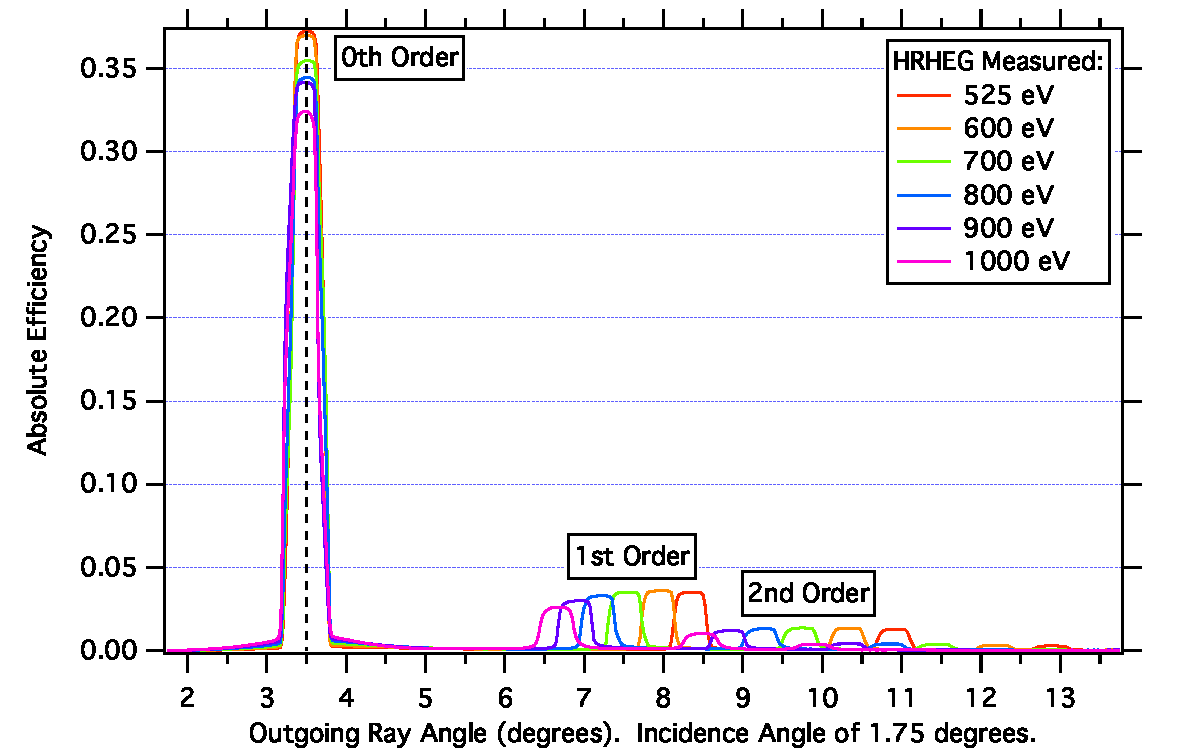
\includegraphics[scale=0.8]{Chapter5/5c_angleScan/5c_solidColors.pdf} 
   \caption[The simplest diffractometer experiment scans the detector angle while illuminating the grating with a constant photon energy.]{The simplest diffractometer experiment scans the detector angle while illuminating the grating with a constant photon energy.  The diffraction orders are visible as peaks along the outgoing angle axis (measured up from the incident beam direction at 0$\deg$).  The 0th order (reflection) peak is easily visible at 3.5$\deg$, or twice the incident angle (88.25$\deg$, or 1.75$\deg$ from grazing).  Grating: HRHEG.}
   \label{5c}
\end{figure}

\begin{figure}[htbp] %  figure placement: here, top, bottom, or page
   \centering
   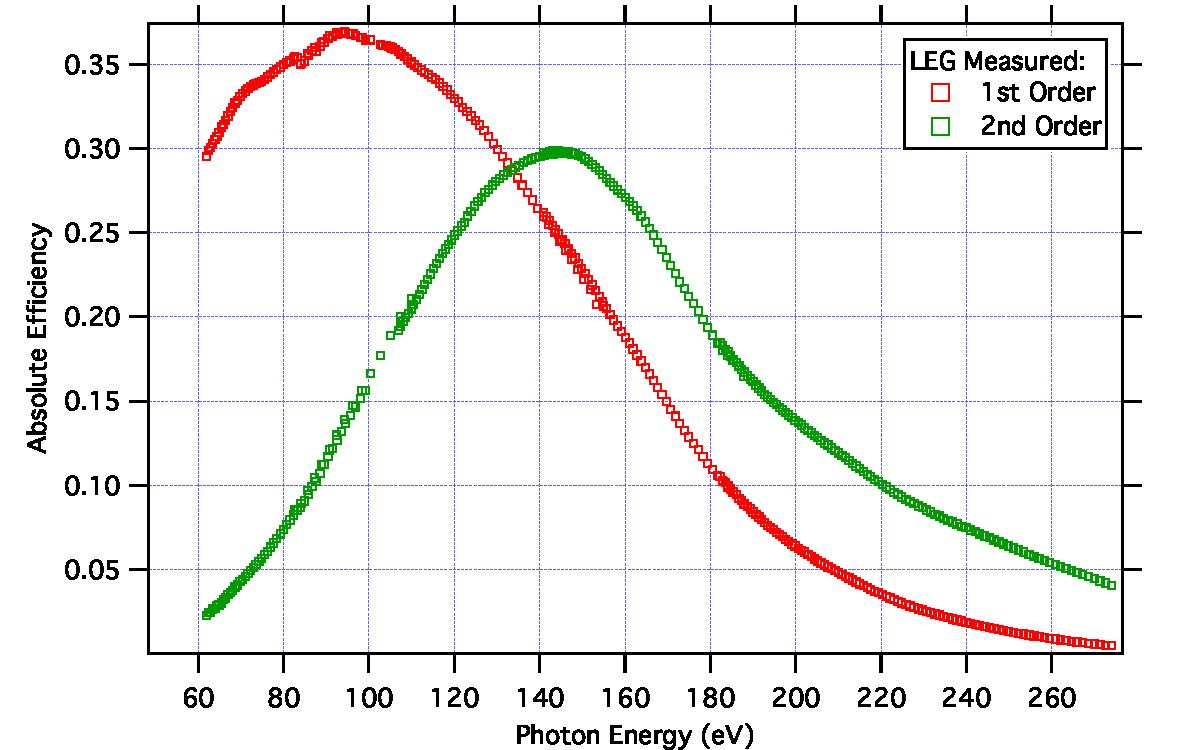
\includegraphics[scale=0.8]{Chapter5/5d_energyScan/5d_LEG.pdf} 
   \caption[When the groove density of a grating is accurately known, the detector angle can be moved in tandem with the monochromator energy to keep it on the diffraction peak as the incident photon energy is scanned.]{When the groove density of a grating is accurately known, the detector angle can be moved in tandem with the monochromator energy to keep it on the diffraction peak as the incident photon energy is scanned.  This allows faster, nearly continuous efficiency measurements as a function of photon energy.  (Grating: LEG)}
   \label{5d}
\end{figure}

\subsubsection{Wavelength calibration}
The monochromator on Beamline 6.3.2 is slitless, therefore its absolute energy calibration is affected by the position of the beam in the ALS storage ring.  To calibrate the energy axis of our data, we scanned the monochromator through the absorption edges of the higher-order suppression filters, and compared the onset of the edges with the published values for the binding energies of these elements:
	\begin{enumerate}
	\item For every new energy range, monochromator grating change, or storage ring refill, the sample was moved out of the way and the photodiode was placed at 0 degrees to measure the direct beam.
	\item The monochromator was scanned upward in energy through the onset of the nearest absorption edge of a filter placed in the beam path.  (For example, prior to doing scans in the energy range from 82.6 to 112 eV, we installed the silicon filter and scanned across the Si $L3$ absorption edge, located at 99.42 eV.)  Essentially, this amounted to measuring a transmission x-ray absorption spectrum of the filter element.
	\item The wavelength shift of the onset of the absorption edge (in monochromator wavelength units) away from its theoretical position provided a correction offset that was applied to the wavelength axis for all scans in this range.\footnote{The monochromator control software used wavelength units rather than energy units, so we conducted all of our efficiency scans in wavelength units and converted later from nm to eV, using the photon energy relationship $E=hc/\lambda$.}
	\end{enumerate}
	
\subsubsection{Normalization}
\label{normalizationEff}
Chapter 3 defined grating efficiency as the ratio of the intensities of the $n$th order diffracted beam and the incident beam.  In our measurement procedure (above), we used the photodiode to record the intensity of the reflected beam $I_r$, and subsequently the intensity of the incident beam $I_i$.  The efficiency $e^{(r)}$ would then be
\begin{align}
e^{(r)} = \frac{I_r}{I_i}
\end{align}
Using the same detector to measure both the reflected and incident beam eliminates error due to differences in detector sensitivity.  However, because these measurements were not taken simultaneously, it is possible that the incident beam intensity would have changed in the interim; in fact, this would be virtually guaranteed due to decay of the storage ring current over time.  Because the light intensity of a bending magnet beamline is proportional to the storage ring current $J_{\mathrm{ring}}$, we can record the ring current at the time of each measurement, and use it to normalize the intensities:
\begin{align}
e^{(r)} = \frac{I_r / J_{\mathrm{ring},r}}{I_i / J_{\mathrm{ring},i}}
\end{align}

Finally, as we identify in the following section, the dominant source of error in low-light photodiode measurements is the \emph{dark current}: an intensity-independent signal from the photodiode that increases with temperature due to thermal generation of electron-hole pairs.  With the beam blocked, we measured the dark current $I_{\mathrm{dark}}$ for every gain setting of the photodiode, and subtracted this  contribution from all measurements to determine the true intensity ratio:
\begin{align}
e^{(r)} = \frac{(I_r - I_{\mathrm{dark}}) / J_{\mathrm{ring},r}}{(I_i - I_{\mathrm{dark}})/ J_{\mathrm{ring},i}}
\label{effNormalization}
\end{align}
We used Eqn. \eq{effNormalization} to normalize all of the efficiency results in Section \ref{gratingResults}.

\subsection{Sources of error}
\label{sourcesOfError}
In the previous description of our procedure, we briefly mentioned the ``higher-order suppressor'', the dark current, and the energy calibration.  In this section, we take a look at all of the sources of error which could affect the grating efficiency measurements.
\subsubsection{Higher-order contamination}
\label{higherOrderContamination}
A bending magnet source like the one on Beamline 6.3.2 produces light of all wavelengths, from infrared to hard x-rays; it is the responsibility of the monochromator to extract a single wavelength from this broadband input.  The problem with grating monochromators, however, is that the grating equation cannot distinguish between equivalent products of $n$ and $\lambda$: light with a wavelength of $x$ nanometers diffracted in 1st order will leave at the same angle as $x/2$-nanometer light diffracted in 2nd order.\footnote{In terms of energy, photons with an energy of $y$ eV will diffract in 1st order to the same angle as $2y$-eV photons in 2nd order.}  When both wavelengths are present in the monochromator input, this creates what is known as ``higher-order contamination'' in the output.  Because the monochromator gratings are likely more efficient in 1st order than any other, the intensity of $x/2$ and $x/3$-nanometer light will be comparatively lower than the desired wavelength, but it will still contaminate the mono output.  If this higher-order light were to arrive at the grating under test, it would be diffracted again, introducing additional erroneous peaks into the detector angle scan.  (Depending on the ratio of the monochromator and test-grating groove densities, these erroneous peaks could either overlap or fall beside the ``true'' diffraction peaks.)  Therefore, reflectometry experiments require a method to eliminate this higher-order light before it reaches the sample.

Beamline 6.3.2 has two techniques for higher-order suppression.  The first is a variable-incidence mirror with multiple sets of coating stripes.  This design exploits the change in reflectivity as a function of incidence angle and energy that we saw (for example) in Figure \ref{reflectionVsAngle}.  Depending on the desired wavelength, the mirror coating and grazing angle are chosen to provide high reflectivity at the desired wavelength, but significantly lower reflectivity at fractionally-shorter wavelengths. (TODO find ref)

The second technique is a filter wheel containing a set of transmission filters from various elements which may be inserted into the beam path prior to the endstation.  The filters are between 300 nm and 1 um thick, and are designed to remove 50\% or more of the light at energies above the filter's absorption edge.

Table \ref{filterTable} shows the mirror coating, mirror angle, and filter element that we used for higher-order suppression.  The energy ranges of each mirror/filter combination (shown in the left column) restricted the maximum extent of each efficiency scan; for the efficiency results shown in Section \ref{gratingResults}, we have combined multiple scans together.

\begin{table}[htbp]
   \centering
   \caption[For higher-order suppression, Beamline 6.3.2 has a variable-incidence mirror and a set of transmission filter elements.  The mirror coating, mirror angle, and filter need to be selected based on the energy range of the scan.]{For higher-order suppression, Beamline 6.3.2 has a variable-incidence mirror and a set of transmission filter elements.  The mirror coating, mirror angle, and filter need to be selected based on the energy range of the scan.  (Mirror angles are measured from grazing incidence.)}
   \begin{tabular}{@{} |c|l|c|l| @{}} % Column formatting, @{} suppresses leading/trailing space
      \hline
Energy Range	(eV) &	Mirror	&	Mirror Angle ($\deg$)	&	Filter	\\
\hline\hline
62 - 99	&	\multirow{4}{*}{Carbon}	&	\multirow{2}{*}{10}	&	Silicon	\\
83 - 112	&			&			&	Beryllium	\\
\cline{3-4}
103 - 155	&			&	8	&	\multirow{2}{*}{Boron}	\\
141 - 188	&			&	6.2	&			\\
\hline
182 - 276	&	\multirow{2}{*}{Nickel}	&	\multirow{2}{*}{8}	&	Carbon	\\
275 - 454	&			&			&	[None]	\\
\hline
441 - 546	&	\multirow{4}{*}{[None]}	&		&	Chromium	\\
544 - 775	&			&		&	Cobalt	\\
751 - 932	&			&		&	Copper	\\
898 -  1305&			&		&	Magnesium	\\
      \hline
   \end{tabular}
   \label{filterTable}
\end{table}

\subsubsection{Monochromator energy calibration}
The monochromator is approximately calibrated, so that entering a wavelength set-point into the control software -- for example, 2.73 nm -- will align the mono grating to diffract light of approximately 2.73 nm out through the exit slit.  However, the calibration is not perfect, and it is also affected by shifts in the ALS electron beam orbit position.  Therefore, it is important to obtain an absolute wavelength calibration whenever moving to a substantially different wavelength range, changing monochromator gratings, or resuming scans after a storage ring refill.

As described in the procedure, we calibrated the wavelength axis of our efficiency scans (eventually, the energy axis) by conducting transmission absorption spectroscopy on the filter elements in Table \ref{filterTable}.  The difference between the monochromator's apparent wavelength at the halfway height of the absorption edge, and the wavelength corresponding to the published binding energies for those elements, was used to generate a wavelength offset for nearby scans.  (The monochromator's calibration might also suffer from errors which require linear and quadratic scaling corrections, but we assumed that a simple offset would be sufficient over the short length of these scans.)

\subsubsection{Photodiode dark current}
Photodiodes can be operated in a forward-biased (\emph{photovoltaic}) mode, or in a reverse-biased (\emph{photoconductive}) mode.  When used as sensitive detectors of light intensity, the photoconductive mode is almost always used, because it offers faster response times and a linear response to light intensity over many orders of magnitude.  In this mode, a reverse bias is applied and -- in the absence of light -- only a small \emph{dark current} flows through the diode, due to the thermal generation of electron-hole pairs in the $p-n$ junction.  When light strikes the $p-n$ junction, incident photons create electron-hole pairs which are swept across the junction by the reverse bias, and create an intensity-dependent \emph{photocurrent}.  The total current through the photodiode is measured by a sensitive current amplifier.

The dark current depends on temperature, and slightly on the magnitude of the reverse bias voltage.  (In our instrumentation, the reverse bias was affected by the gain setting of the current amplifier.)  To account for this, we measured the dark current at every gain setting with the beam turned off, and then subtracted this in the normalization equation (Eqn. \eq{effNormalization}).  The dark current measurements were conducted after the diode had been operating under reverse bias for some time (and hopefully had reached operating temperature).  Since the dark current increases with temperature, it is possible that exposure to extreme intensity would heat the detector and change the dark current contribution; however, this effect should be negligible for the low intensities observed in our experiment.

\subsubsection{Saggital tilt of the grating}
The reflectometer mechanics enable the intended rotation of the sample (grating) around the $x$-axis in FIgure \ref{reflectometerCoordinates}.  If the grating surface were tilted away from normal incidence around the $y$-axis -- either due to an offset in the grating mount, or due to the curvature of the grating combined with incorrect alignment in the $x$-direction -- light would be reflected out of the $y-z$ plane.  This would create the ``conical mount'' situation we assumed we could avoid modelling in Chapter 3, and would also cause the diffracted beam to partially or completely miss the 2 mm pinhole of the photodiode detector.  Both of these effects would reduce the observed intensity from what we would expect.

The zero-order alignment test we described in the procedure confirmed that with the grating positioned at 2 degrees, a substantial current was observed on the photodiode at 4 degrees, indicating that a substantial amount of light was staying within the plane of incidence.  However, we cannot confirm that the alignment was flawless, and it is possible that the measured efficiencies are lower than they would be under perfect alignment.

\subsubsection{Limited beam spot size}
The Beamline 6.3.2 optics focus the beam to a spot size of 0.010 mm x 0.3 mm on the grating.  (TODO check if we were focussed at grating or infinite.)  Because the grating needs to be aligned on the centre of rotation, there can only be one position for the beam on the grating, and so we could only test the efficiency at this point.  If there is variation in the groove profile across the grating, the illuminated part of the grating may not actually be representative of the average efficiency.  

It is impossible to overcome this limitation; even if it were possible to fully illuminate the grating, the grating curvature would not be correct to focus the diffracted beam to the same size on the detector as the incident beam would be.  Therefore, a small beam size is a necessary compromise to minimize the focussing effect of the grating.

\subsubsection{Energy dispersion across detector pinhole (finite size of pinhole + finite resolution dE)}
TODO need to discuss with Eric Gullikson
\subsubsection{Focussing / Defocussing}
TODO need to discuss with Eric Gullikson

\section{Real-world grating effects}
\label{realWorldEffects}
The comparisons between the predicted and measured efficiencies for each grating are discussed in Section \ref{gratingResults}, and impatient readers might have already beat us there.  However, before looking at the results, it might be useful to consider some of the factors that could cause a discrepancy between the two.  If there are differences between the predicted and measured efficiency, this would imply one -- or more -- of three distinct possibilities:
\begin{enumerate}
\item That the measurement procedure, due to experimental error, did not measure the actual grating efficiency.
\item That the theory and calculation method do not correctly describe the gratings they attempted to model,\\
or,
\item That the real-world gratings, as produced, are different from the ones we modelled.
\end{enumerate}
We dealt with the first possibility in the previous section on sources of error.  Before accepting the second possibility, we take a look at some of the ways manufactured gratings differ from ideal ones.

\subsection{Stray radiant energy}
For a perfectly periodic surface, the Rayleigh expansion in Chapter 3 showed that all of the light propagating away from a grating leaves as plane waves in discrete orders. Regardless of the groove shape, no light leaves except at the angles given by the grating equation (Eqn. \eq{gratingEquation}).  In real-world gratings, deviations from perfect periodicity lead to \emph{stray radiant energy} (SRE), which is a general term for all radiation that leaves at other angles.  (TODO REF http://gratings.newport.com/information/technotes/technote9.asp) Due to conservation of energy, the more SRE that exists, the less energy there is in the desired orders, and the lower the grating efficiency.  SRE also affects the resolution of a grating instrument, by increasing the background noise level and contaminating the outgoing angles with light of the wrong wavelength.

Stray radiant energy can be caused by microroughness of the grating surface, variation in the height or spacing from groove to groove, and other imperfections such as dust and scratches.
\subsubsection{Surface roughness}
The grating model in Chapter 3 assumed a perfectly smooth surface, given by the periodic profile $y=g(x)$ in Figure \ref{2a}.  Unfortunately, both ruling and coating processes invariably leave a certain amount of microroughness, shown exaggerated in Figure \ref{5e}.  When the surface is rough on the scale of the incident wavelength, it causes diffuse scattering, which is analogous to the diffuse (or non-specular) reflection that would occur off any rough surface.  Because this phenomenon affects the entire  area of the grating, diffuse scattering from surface roughness is typically responsible for most of the reduction in real-world grating efficiency (compared to theoretical calculations).

\begin{figure}[htbp] %  figure placement: here, top, bottom, or page
   \centering
   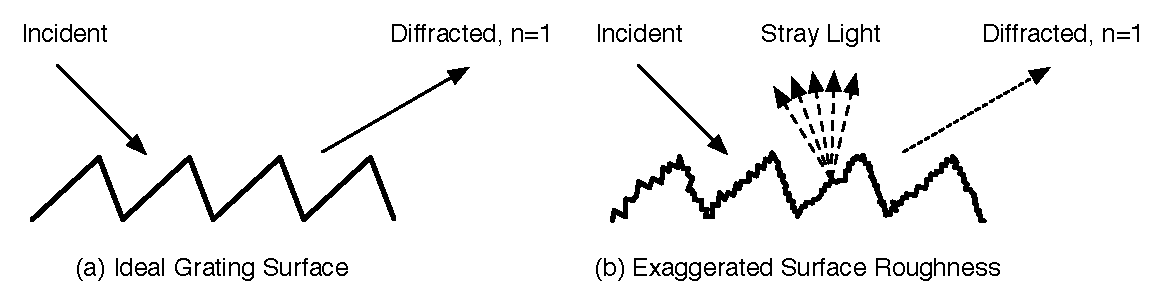
\includegraphics[scale=0.8]{Chapter5/5e_surfaceRoughness/5e.pdf} 
   \caption{Roughness of the grating surface scatters stray light outside the diffraction orders. Typically, surface roughness is responsible for most of the reduction in real-world grating efficiency, compared to theoretical calculations.}
   \label{5e}
\end{figure}
 
Although it might not be clear from Figure \ref{5e} -- which is two-dimensional -- diffuse scattering need not be constrained to the plane of incidence. The roughness creates slope variation in both $x$ and $z$, so scattered light could end up anywhere in the hemisphere above the grating.  However, in-plane scattering is stronger than out-of-plane scattering by a factor of $1/\cos\theta$ (where $\theta$ is the incidence angle from normal). Therefore, at grazing incidence, the in-plane scattering is dominant. (TODO REF http://www2.astro.psu.edu/~niel/astro485/xrayschool/schwartz-xray\_optics.pdf)

To correct the predicted grating efficiencies for scattering, we need to understand two things:
\begin{enumerate}
\item The amount of energy lost to scattering, as a function of roughness, wavelength, incidence angle, and diffraction order.
\item The angular distribution of the scattered intensity. Does it affect all diffraction orders the same way?
\end{enumerate}

Given the randomness of the surface structure, we need statistical methods to answer these questions.  Statistically, the surface roughness is characterized by $\sigma$, the root mean square (RMS) variation in height from the nominal plane, and by the power spectral density (PSD) function, which describes how the height variation is distributed in frequency.
%\footnote{Because the surface height is ``stationary random process'' -- i.e.: the mean and variance do not change over position -- the PSD is the Fourier transform of the autocorrelation function of the height $h(x)$.}

Even for the simpler (non-grating) case of roughness on flat surfaces, a substantial amount of research has only succeeded in producing a murky swamp of approximate models. (TODO REF Elfouhaily and Guerin) categorized 260 references -- 177 since 1980 -- into 30 different methods, before concluding that ``there does not seem to be a universal method that is to be preferred systematically. All methods present a compromise between versatility, simplicity, numerical efficiency, accuracy and robustness, with a different weighting in these various fields. [...] No approximate model has fulfilled all listed criteria''

Even though they only deal with nominally flat surfaces, all of these methods are based on the assumption that a random rough surface can be decomposed into a superposition of sinusoidal gratings\footnote{Obviously, in our case, of much higher groove density than the actual gratings!}, and that scattering can be explained as a diffraction effect from the phase changes created by the ``microtopography'' of the surface.  (TODO REF Modified Beckmann-Kirchhoff scattering model for rough surfaces with large incident and scattering angles
Opt. Eng. 46, 078002 (Jul 02, 2007); doi:10.1117/1.2752180)  There are two fundamental approaches: the Rayleigh-Rice theory (TODO REF Lord Rayleigh, �On the Dynamical Theory of Gratings�, Proc. Roy. Soc. A79, 399-416 (1907)., S. O. Rice, �Reflection of Electromagnetic Waves from Slightly Rough Surfaces�,Commun. Pure Appl. Math., vol. 4, 1951, p.351., ), which is a perturbation approximation for solving the electromagnetic vector wave equation near periodic interfaces, and the Beckmann-Kirchoff theory, which uses a scalar wave equation and applies the Kirchoff diffraction formula (TODO REF P. Beckmann and A. Spizzichino, The Scattering of Electromagnetic Waves from Rough Surfaces; Pergamon, New York, 1963, Chaps. 4 and 5.).  Both contain approximations; the Rayleigh-Rice methods are only applicable to ``smooth'' surfaces, where the perturbation from a flat surface is small -- i.e., where the RMS roughness is small compared to the wavelength ($\sigma \ll \lambda$).  The Beckmann-Kirchoff methods are appropriate for ``rougher'' surfaces up to $(\sigma \cos \theta \leq \lambda)$, but they contain a small-angle approximation that restricts them to near-normal incidence and scattering angles (TODO REF modified).  (In the extreme case where the roughness is much larger than the wavelength, it becomes more appropriate to handle it using a geometric optics approach, rather than a diffraction approach.  In this situation, we can imagine a surface made up of many ``microfacets'' all reflecting light at different angles; the BESSY raytracing software suite actually uses this approach to model roughness by randomly varying the direction of a mirror's normal vector (slightly) for each reflecting ray, according to the statistical description of the surface (TODO REF bessy RAY paper.)

Since grating theories are already being used to describe diffuse scattering from rough \emph{flat} surfaces, applying these methods to \emph{actual} gratings is even more difficult; this amounts to creating a superposition of (very high density) gratings, \emph{on the surface of a grating}(!)
 
 It would be theoretically difficult to analyze ``gratings structured on top of gratings'', so instead, we apply some of the results for rough mirrors to come up with an approximate correction for our grating efficiencies.  Many texts and computer programs use a simple expression called the ``Beckmann factor''
\begin{align}
R' &= R \exp\left(  - \left(\frac{4\pi\sigma \,  \cos \theta}{\lambda}\right)^2    \right)
\end{align}
to approximate the reflectivity $R'$ of a real mirror, where $R$ would be the reflectivity of an ideally smooth surface.  However, this is subject to the small-angle approximation in the Beckmann approach, and predicts that the reflectivity is essentially unchanged  when approaching grazing incidence due to the $\cos^2\theta$ term in the exponential. 
 
 Based on a the x-ray-specific work of (TODO REF http://link.aps.org.cyber.usask.ca/doi/10.1103/PhysRevB.38.2297), the X-ray Data Booklet (TODO REF) gives a correction factor of
\begin{align}
R' &= R \exp\left(  - \left(\frac{4\pi\sigma}{\lambda}\right)^2 \sin \theta \, \mathbf{Re}\left[ \sqrt{n^2 - \sin^2 \theta}  \right]    \right)
\end{align}
where $n$ is the complex refractive index.\footnote{TODO REF gives the complex reflection coefficient, instead of the reflectivity.  Compared to the expression given there, we have converted from grazing incidence angles to normal incidence angles, and multiplied by the complex conjugate to determine the reflectivity.}  This was derived from the ``distorted-wave Born approximation'', which uses a Rayleigh-Rice-like perturbation approach; it is far more accurate in the limit of grazing incidence.

By analogy from reflectivity (``fraction of incident light reflected'') to grating efficiency (``fraction of incident light reflected in order $n$''), we have used the same factor to determine the form of the roughness correction to apply to the grating efficiencies:
\begin{align}
e_n' &= e_n \exp\left(  - \left(\frac{4\pi\sigma}{\lambda}\right)^2 \sin \theta \, \mathbf{Re}\left[ \sqrt{n^2 - \sin^2 \theta}  \right]    \right)
\label{roughnessCorrection}
\end{align}
Since we do not have measurements of each grating's RMS roughness, we used $\sigma$ as a free parameter to attempt to fit the theoretical efficiencies to the measured efficiencies; the results are shown in Section \ref{gratingResults}.

Although we do use this mirror expression to correct our predicted efficiencies, it is important to note that roughness on gratings may actually cause different effects than roughness on flat mirrors.  (TODO REF http://www.gratinglab.com/information/handbook/chapter10.asp\#10.1.1) reports that the diffuse scattering is not isotropic; within the plane of incidence, the intensity is stronger at angles near the diffraction orders than it is between orders.  (TODO REF M. R. Sharpe and D. Irish, "Stray light in diffraction grating monochromators," Opt. Acta 25, 861-893 (1978)) analyzes scattering specifically from gratings, and indicates that the intensity of scattering increases as the fourth power of the energy.  (TODO REF Angular distribution of light scattered from a sinusoidal grating 1 September 2000 Vol. 39, No. 25 APPLIED OPTICS) looks at sinusoidal gratings illuminated by coherent visible light, and confirms that surface roughness increases the background light level. (TODO REF L. Nevot, P. Croce, Rev. Phys. Appl. 15, 761 (1980). 10.1051/rphysap:01980001503076100) provides another comprehensive study of rough gratings, and comes to a result consistent with Sinha et. al. (Eqn. \eq{roughnessCorrection}), although through a different method.

Figure TODO shows the reduction in efficiency caused by different amounts of roughness, over the range of soft x-ray energies.  These were calculated at grazing incidence using the Sinha approach, so we are limited to RMS roughnesses much smaller than the wavelength.  The Beckmann (Eqn. \eq{beckmannFactor}) and Sinha (Eqn. \eq{roughnessCorrection}) factors are compared in Figure TODO, showing the limits of each one's applicability.

Figure TODO reinforces how important it is to keep the roughness low during manufacturing.  Our AFM measurements suggest that re-coating the grating after ruling adds to the roughness, due to the granular nature of the evaporated coating.  Due to extensive manufacturing experience, gold coatings are usually the smoothest to apply -- as was the case for our LEG.  The subsequent platinum and nickel overcoatings on the remaining gratings resulted in a much rougher surface.

\subsubsection{Dust, scratches, and pinholes}
Dust, scratches, pinholes, and any other out-of-place bumps on the surface also contribute to the stray radiant energy.  All of these features act as scattering centres and create diffuse light; we can easily confirm this for visible wavelengths (using our biological photodetectors) when looking at a dirty grating under bright light.  Given the challenges of modelling statistically well-behaved surface roughness, we do not even attempt to model these purely random defects, beyond recognizing that they will reduce the overall grating efficiency and contribute to stray light.

\subsubsection{Periodic irregularities of the grooves: ghost peaks}
In the section on grating manufacturing (Section \ref{gratingManufacturing}), we mentioned that periodic errors in the groove position or groove height will create ``ghosts'': additional light intensity peaks superimposed over the desired diffraction pattern.  This happens because the higher-order structure acts like a superimposed grating with its own periodicity.  Just like the other causes of stray radiant energy, these peaks -- if present -- will remove energy from the desired diffraction orders, and contaminate the resolution by directing light to the ``right place at the wrong wavelength''.

\subsubsection{Irregularities along the groove: out-of-plane reflection}
We assumed in Chapter 3 that the grating was invariant (i.e., did not change) along the $z$ direction of the grooves.  When ruling a mechanical grating, changes in the elasticity of the metal will allow the tip to penetrate to different depths, causing variation in the shape of the profile along the grooves.  (This also occurs with holographic gratings, due to variation in the mean intensity of the interference pattern during exposure.)  Shape variation along the grooves can reflect light out of the plane of incidence, and the effect can be diffuse or specular. 

Elasticity changes will also cause random (non-periodic) variation in the groove depth from groove-to-groove.  This has been shown to create a continuous distribution of scattered light which increases as a function of $(1/\lambda^3)$ (TODO REF M. R. Sharpe and D. Irish, "Stray light in diffraction grating monochromators," Opt. Acta 25, 861-893 (1978).)

\subsection{Manufacturing errors the \emph{can} be modelled}
All of the previous real-world grating flaws -- surface roughness, dust and scratches, periodic and non-periodic groove irregularities -- represent deviation from the theoretical profile we modelled in Chapter 3, in ways that cannot be incorporated into the model without breaking our initial assumptions (Section \ref{s_assumptions}).  It is also possible for manufacturing errors to create deviation that we \emph{can} actually model; the best example of this would be differences between the requested and manufactured groove geometry.
\subsubsection{Profile errors: Blaze angle errors shift the efficiency peak}
Figure \ref{3i-2} showed how small (0.1$\deg$) changes in the blaze angle can significantly shift the efficiency peak.  For mechanically-ruled gratings, the accuracy of the blaze angle depends on the persistence and perfectionism of the ruling engine operator, who must adjust the diamond tip angle during setup through tedious trial-and-error.  If, after manufacturing, the real blaze angle turns out to be different than what the customer specified -- always true to some degree -- we can measure the true blaze angle using a calibrated AFM, and re-calculate the theoretical efficiencies using a better approximation of the profile.

Alternatively, if calibrated AFM measurements are not available, we have determined that the shape of the measured efficiency curves and the ratio between 1st and 2nd order efficiency can provide a strong indication of the real blaze angle.  (For example, by choosing the best-fit blaze angle to match the measured and calculated efficiency curves, we predicted a blaze angle of 2.0$\deg$ for the MEG grating, before determining from AFM measurements that the real blaze angle was 2.04$\deg$.)  In Section \ref{gratingResults}, we discuss the blaze angle agreement for each grating.

The same techniques can be applied to profiles other than blazed gratings; the first method works as long as the groove geometry (Figure \ref{3c-profile}) can be measured.  For profiles like trapezoidal gratings that have three -- instead of just one -- adjustable parameters, it becomes more involved to try to estimate the best-fit geometry, but this can be accomplished using multidimensional minimization algorithms.

\subsubsection{Coating oxidation changes the reflectivity spectrum}


\begin{figure}[htbp] %  figure placement: here, top, bottom, or page
   \centering
   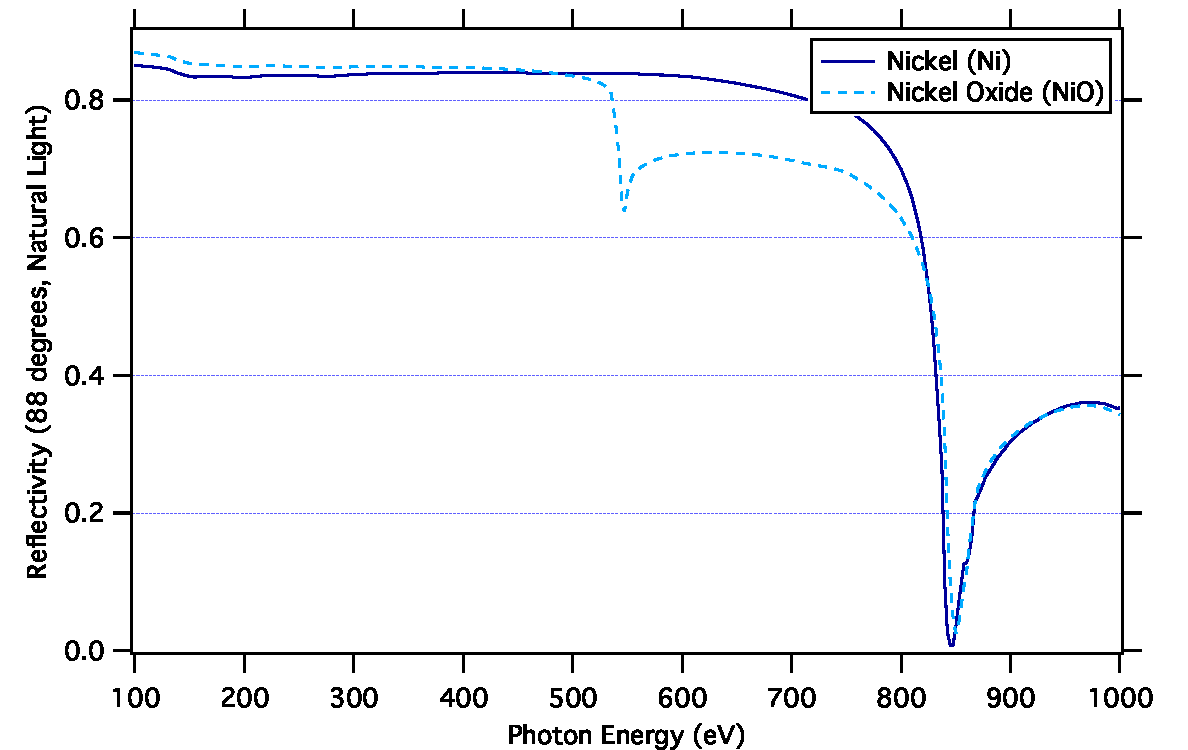
\includegraphics[scale=0.8]{Chapter5/5f_oxidized/Ni_NiO_reflec.pdf} 
   \caption{Unprotected Nickel quickly forms a surface oxide of NiO, which strongly reduces the reflectivity at the Oxygen edge (525eV) }
   \label{5f}
\end{figure}

\section{Grating results}
\label{gratingResults}
   : (and comparison to theoretical)
\subsection{LEG} (gold): profile clean; as expected; blaze angle off. [modelled]

\begin{figure}[htbp] %  figure placement: here, top, bottom, or page
   \centering
   \includegraphics[scale=0.8]{Chapter5/5y_afm/LEG.pdf} 
   \caption{AFM measurements of the Low Energy Grating (LEG) profile, averaged along the grooves (TODO um x TODO um).  The best-fit blaze angle is at the centre of the grating.}
   \label{5y-leg}
\end{figure}

\begin{figure}[htbp] %  figure placement: here, top, bottom, or page
   \centering
   \includegraphics[scale=0.8]{Chapter5/5x_comparison/LEG.pdf} 
   \caption{Theoretical and measured efficiency of the Low Energy Grating (LEG).}
   \label{5x-leg}
\end{figure}


\subsection{IMP} (nickel): Profile clean, blaze angle off [modelled].  Oxidized� Modelled as NI, layer of NiO.

TEST: NiO on top of Ni? layer thickness
Caveat: Henke data reflectivities are not correct at/near absorption edges... shouldn't totally match theoretical shape.

          - compare AFM and fitted
          
          scattering factor: http://www2.astro.psu.edu/~niel/astro485/xrayschool/schwartz-xray\_optics.pdf --> 1/sin(theta)

\begin{figure}[htbp] %  figure placement: here, top, bottom, or page
   \centering
   \includegraphics[scale=0.8]{Chapter5/5y_afm/IMP.pdf} 
   \caption{AFM measurements of the Impurity Grating (IMP) profile, averaged along the grooves (TODO um x TODO um).  The best-fit blaze angle is at the centre of the grating.}
   \label{5y-imp}
\end{figure}

\begin{figure}[htbp] %  figure placement: here, top, bottom, or page
   \centering
   \includegraphics[scale=0.8]{Chapter5/5x_comparison/IMP.pdf} 
   \caption{Theoretical and measured efficiency of the Impurity Grating (IMP).}
   \label{5x-imp}
\end{figure}


\subsection{MEG} (nickel): profile ok, blaze angle off [modelled].  Oxidized� Modelled as combination of NiO and NiO2.

\begin{figure}[htbp] %  figure placement: here, top, bottom, or page
   \centering
   \includegraphics[scale=0.8]{Chapter5/5y_afm/MEG.pdf} 
   \caption{AFM measurements of the Medium Energy Grating (MEG) profile, averaged along the grooves (TODO um x TODO um).  The best-fit blaze angle is at the centre of the grating.}
   \label{5y-meg}
\end{figure}

\begin{figure}[htbp] %  figure placement: here, top, bottom, or page
   \centering
   \includegraphics[scale=0.8]{Chapter5/5x_comparison/MEG.pdf} 
   \caption{Theoretical and measured efficiency of the Medium Energy Grating (LEG).}
   \label{5x-meg}
\end{figure}

\subsection{HEG} (Pt): almost no diffraction performance at all. AFM: revealed double-peak structure; not ruled correctly. Sent back to manuf.

\begin{figure}[htbp] %  figure placement: here, top, bottom, or page
   \centering
   \includegraphics[scale=0.8]{Chapter5/5y_afm/HEG.pdf} 
   \caption{AFM measurements of the High Energy Grating (HEG) profile, averaged along the grooves (TODO um x TODO um).  Severe ruling errors were apparent.  The profile wasn't sufficiently triangular to attempt to fit a blaze angle.}
   \label{5y-heg}
\end{figure}

\begin{figure}[htbp] %  figure placement: here, top, bottom, or page
   \centering
   \includegraphics[scale=0.8]{Chapter5/5x_comparison/HEG.pdf} 
   \caption{Theoretical and measured efficiency of the High Energy Grating (LEG).}
   \label{5x-heg}
\end{figure}

\subsection{HRMEG and HRHEG}

\begin{figure}[htbp] %  figure placement: here, top, bottom, or page
   \centering
   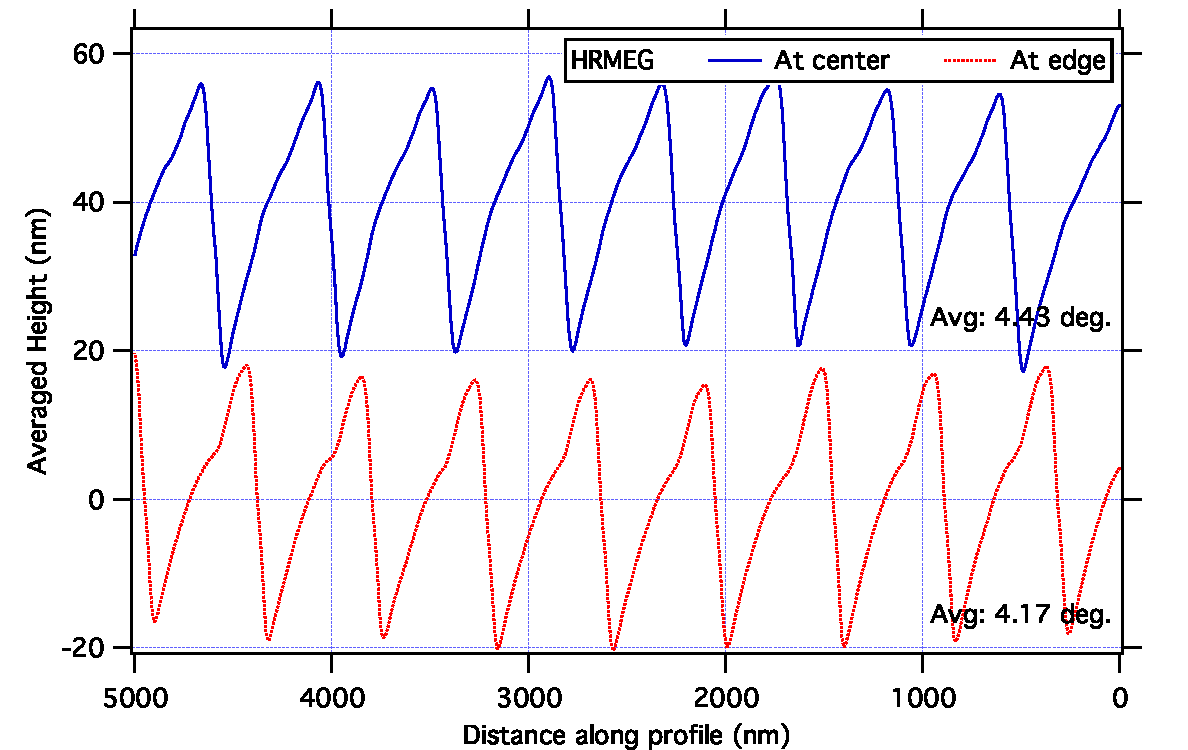
\includegraphics[scale=0.8]{Chapter5/5y_afm/HRMEG.pdf} 
   \caption{AFM measurements of the HighRes Medium Energy Grating (HRMEG) profile, averaged along the grooves (TODO um x TODO um).  The best-fit blaze angle is at the centre of the grating.}
   \label{5y-hrmeg}
\end{figure}

\begin{figure}[htbp] %  figure placement: here, top, bottom, or page
   \centering
   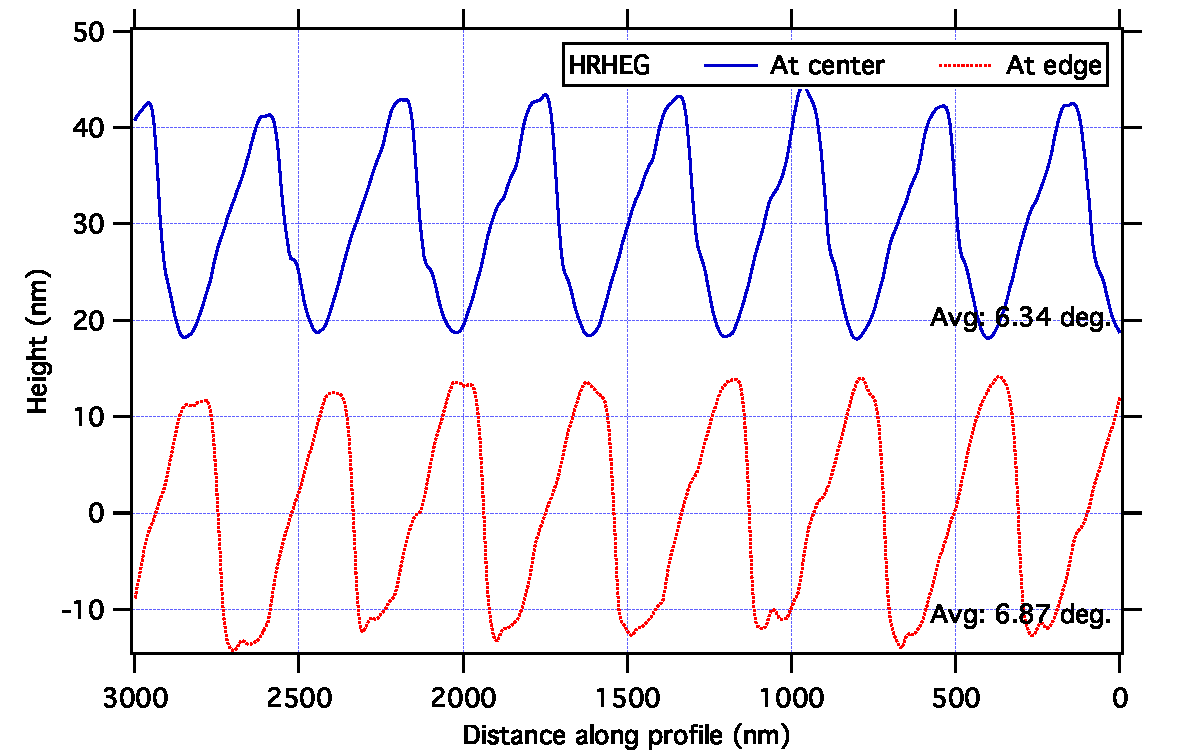
\includegraphics[scale=0.8]{Chapter5/5y_afm/HRHEG.pdf} 
   \caption{AFM measurements of the HighRes High Energy Grating (HRHEG) profile, averaged along the grooves (TODO um x TODO um).  The best-fit blaze angle is at the centre of the grating.}
   \label{5y-hrheg}
\end{figure}




 (Pt): blaze angles very off� Unsuitable for actual application in 3rd order.
          - Temporary plan: Using HRHEG (2600l/mm) in place of HEG (2000l/mm) since blaze angle error makes it suitable for use in 1st order.
               - DATA 5q: plot expected reduction in efficiency
               
